\documentclass[12pt]{article}

\usepackage[letterpaper, margin=1in]{geometry}
\usepackage{amsmath}
\usepackage{graphicx}
\usepackage{subfigure}

\title{Depth correction for virtual objects enclosed by 360 video}
\author{Liu Jiacheng}

\begin{document}

\maketitle

\section{Basics}

When viewing 360 video in virtual reality, our depth cue is dominated by the monocular cue provided by the video, and binocular cue diminishes. Consequently, an object that is physically on the ground may not be perceived as on the ground. I propose an algorithm for depth correction of virtual objects enclosed in 360 video. \\

In virtual reality, the 360 video is displayed on an inverted sphere of radius $R$ centered at $(0, H_C)$. The ground is plane $y = 0$. For an object on the ground at point $G$, we would like to place it at point $G'$ in order to conform with the depth cue given by the 360 video. For an object on segment $V-G$, we would like to uniformly stretch its position to $V-G'$. \\

Denote $H_V$ as the height of viewer's eyes with respect to ground, $H_O$ as the height of an object with respect to ground, and $r$ as the horizontal distance between the object and the viewer's eyes. For simplicity we now assume $H_C = H_V$. Denote $\theta$ as the angle between segment $V-G$ and the vertical line. 

\begin{align*}
	\theta &= \arctan{\frac{r}{H_V - H_O}} \\
	G' &= (R\sin{\theta}, H_V - R\cos{\theta}) \\
	O' &= (R\sin{\theta} \frac{H_V - H_O}{H_V}, H_V - R\cos{\theta}\frac{H_V - H_O}{H_V})
\end{align*}

Environment: environ scene rendered by 360 image/video
Real object: 
Observed object: 
Projection

\section{Retaining Stationarity of Grounded Objects}

If position tracking is enabled in VR \footnote{Simply disabling position tracking is not a good idea since viewer should be able to translate relative to virtual objects; plus it may introduce vection. }, the viewer's position does not necessarily coincide with the camera's position. As a result, the projected location of observed object will move in accordance to the viewer's movement (but in opposite direction). Since the environment does not move in opposite direction of the viewer, the observed object will be perceived to move relative to the environment. \\

However, when making correction to an object placed stationary on the ground (e.g. an avatar), it would be an apparent artifact if the observed object moves relative to the ground when the viewer moves. Therefore, a projection formula independent of viewer's position is needed, and we choose camera's position as the standard viewer's position in determining the projected position. \\

\begin{figure}[h]
	\centering
	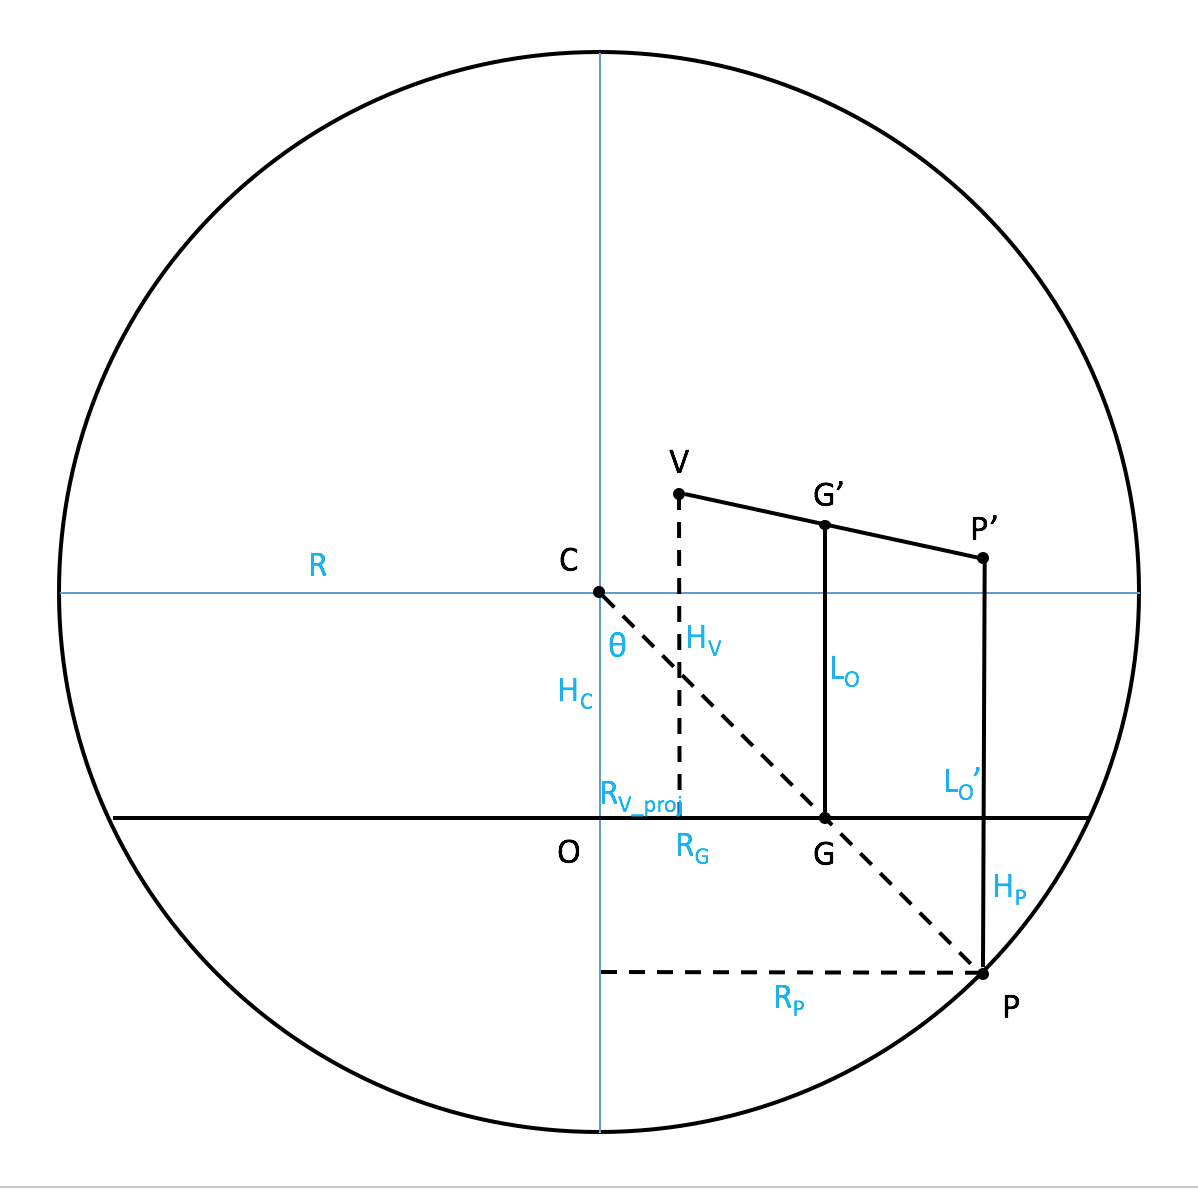
\includegraphics[scale=0.4]{lateral.png}
	\caption{VR scene schema, lateral view. Large circle is environment canvas, $C$ is camera, $V$ is viewer, $G$ is ground position, $P$ is projected position, $GG'$ is real object, $PP'$ is observed object. }
\end{figure}

Use the vertical projection of camera on ground as the origin. The environment is displayed on an inverted sphere centered at camera. Consider the lateral view of the object. Denote $H_C$ as the height of camera, $R_G$ as the horizontal distance between real object and camera, $R_P$ as the horizontal distance between observed object and camera, and $H_P$ as the (signed) vertical distance of observed object from ground. 
\begin{align*}
	\theta &= \arctan{\frac{R_G}{H_C}} \\
	P &= (R \sin{\theta}, H_C - R \cos{\theta})
\end{align*}

Then we need a corresponding scaling formula. Denote $H_V$ as the height of viewer, $R_{V_{proj}}$ as the horizontal distance of viewer from camera, projected onto the lateral plane; $L_O = |GG'|$ as the known height of real object, $L_O' = |PP'|$ as the height of observed object. The scaling factor is $\frac{L_O'}{L_O}$. 
\begin{align*}
	P' &= (R \sin{\theta}, \frac{H_V (R_P - R_G) + L_O (R_{V_{proj}} - R_P)}{R_{V_{proj}} - R_G}) \\
	L_O' &= \frac{H_V (R_P - R_G) + L_O (R_{V_{proj}} - R_P)}{R_{V_{proj}} - R_G} - (H_C - R \cos{\theta})
\end{align*}

\section{Smooth Transition from Grounded Objects to Floating Objects}

When the upper part of the 360 image/video is the sky, depth correction need not be corrected. Also, the above correction formula does not behave well when $(H_O - H_V) \rightarrow 0$. Therefore, we want to enable correction when $(H_O - H_V)$ is below a certain vertical threshold ($-0.1m$). \\

However, if we use a hard threshold, when the object moves upwards, it undergoes sudden transition from corrected mode to uncorrected mode, providing binocular divergence instantaneously and thus make user uncomfortable. It is conceivable that a linear interpolation (wrt position and scale) between real object and observed object also produces a valid imagery of the object. For object below vertical threshold, 
\begin{align*}
	\lambda &= \frac{H_O}{H_C - 0.1m} \\
	Pos_{obs}' &= \lambda Pos_{real} + (1 - \lambda) Pos_{obs} \\
	Scale_{obs}' &= \lambda Scale_{real} + (1 - \lambda) Scale_{obs}
\end{align*}

\section{Strengthen Photorealism by shadowing}

\end{document}
